\documentclass[../Main.tex]{subfiles}% Vietnam green
\begin{document}
	\section{World UBIs Quantitative Data}
	
	To establish a comprehensive understanding of the global landscape of University-Based Incubation Programs (UBIs), it is essential to draw upon quantitative data sourced from reputable international reports, surveys, and academic studies. Such macro-level data not only illuminates general trends and common characteristics but also provides a valuable benchmark for analyzing the specific context of Vietnam.
	
	The prevalence and scope of UBIs worldwide have been extensively documented in UBI Global's World Benchmark Studies and Community Reports, which offer a longitudinal perspective on the evolution of these programs. The 2019-2020 UBI Global World Benchmark Study, for instance, initially assessed 1,580 programs across 82 countries, ultimately retaining 364 programs for its rigorous benchmarking process \autocite{ubi2019world}. This study underscored the widespread presence and high performance of university-linked business incubation and acceleration initiatives, with 41\% of the final sample classified as "World Top University Business Incubators" and 10\% as "World Top University Business Accelerators" \autocite{ubi2019world}. The selection process and classification results are visually summarized in Figure~\ref{fig:ubi_benchmark_flow}, which illustrates the progression from initial assessment to final categorization.
	
	A subsequent shift in the scope of benchmarking is evident in the 2021-2022 UBI Global World Benchmark Study, which adopted a more focused approach by including 109 business incubators and accelerators from 56 countries \autocite{ubi2021world}. This reduction in sample size likely reflects a more stringent selection process or a strategic focus on top-tier programs, as well as possible changes in participation rates.
	
	The 2023 UBI Global Community Report further expands the perspective, revealing that as of March 2023, the UBI Global network encompassed over 1,000 business accelerators and incubators in more than 90 countries \autocite{Amin2024Incubators}. The report highlights the diversity of program types, sectoral focuses, and regional participation, with the United States, Canada, India, the United Kingdom, and Brazil emerging as the top member countries by program count. Regionally, Europe, Asia-Pacific, and North America account for the largest shares of programs, followed by Latin America, Africa, and the Middle East \& North Africa. The sectoral distribution is equally diverse, with significant representation in Health \& Fitness, Green \& Energy, Creative \& Cultural, and Materials \& Manufacturing sectors. Incubators constitute the majority of program types (53\%), followed by accelerators (27\%) and hybrid models (20\%). Notably, university-based programs represent 60\% of the total, underscoring the central role of academic institutions in the global incubation ecosystem.
	
	The top industries served by these programs include HealthTech, IT-services, B2C, Edtech, and Renewable Energy, as depicted in Figure~\ref{fig:top_industries}. In terms of technological trends, Artificial Intelligence, Big Data, Digital Health, Machine Learning, and the Internet of Things are most prominent among supported startups (see Figure~\ref{fig:technology_trends}). Programs cater to startups at various stages of development, with 25\% focusing on the idea stage, 31\% on early stage, and the remaining 44\% split equally between growth and acceleration stages (Figure~\ref{fig:startup_stages}).
	
	A comparative analysis of the benchmark studies from 2019-2020, 2021-2022, and 2023 reveals a notable change in the scope and focus of UBI Global's assessments. While the number of programs and countries included in the formal benchmarking process decreased significantly—from 364 programs in 82 countries to 109 programs in 56 countries—the broader community of business incubators and accelerators has continued to expand, with over 1,000 programs in more than 90 countries by 2023. This trend suggests that, despite increased selectivity in formal benchmarking, the global ecosystem is both growing and diversifying, adapting to emerging trends and regional needs (Figure~\ref{fig:ubi_change_tendency}).
	
	In evaluating the impact and performance of UBIs, UBI Global employs a comprehensive methodology centered on 21 Key Performance Indicators (KPIs), consistently applied across both the 2019-2020 and 2021-2022 benchmark studies \autocite{ubi2019world, ubi2021world}. These KPIs are systematically grouped into three principal categories, each contributing equally to the Program Impact and Performance Score (PIPS). The first category, Value for Ecosystem, assesses the economic impact of programs and their client or alumni startups, as well as their effectiveness in retaining human capital and ventures within the innovation ecosystem. This includes metrics such as jobs created and sustained, sales revenue, graduate outcomes, and self-generated revenue, as well as the retention of client startups and graduates. The second category, Value for Client Startups, evaluates the quantity and efficiency of services provided, the facilitation of community and network building, and access to funding and partnerships. Metrics in this category encompass services offered, coaching and mentoring hours, investment attracted, and alumni engagement. The third category, Value for Program, measures the program's attractiveness to applicants and sponsors, as well as the post-graduation performance of supported startups, including survival rates, the emergence of high-growth enterprises, and successful exits. While these KPIs provide a robust framework for benchmarking and ranking, the reports primarily focus on comparative performance rather than presenting aggregate global data for all metrics.
	
	UBI Global's world rankings consistently highlight top-performing university business incubators, recognizing their outstanding impact and value creation. For the 2019-2020 period, leading incubators included Chalmers Ventures (Sweden), The DMZ at Ryerson University (Canada), IPN Incubadora (Portugal), PoliHub (Italy), The SETsquared Partnership (UK), University of Toronto Entrepreneurship (Canada), UtrechtInc (Netherlands), and YES!Delft (Netherlands) \autocite{ubi2019world}. In the 2021-2022 sample, prominent incubators featured the Center for Technology Development at the University of Brasilia (Brazil), CEI UCN at Universidad Catolica del Norte (Chile), EUREKA at University of Chile (Chile), the Innovation, Business, and Economy Center at the Autonomous University of Baja California (Mexico), King Abdullah University of Science and Technology (Saudi Arabia), MCB at Federal University of Campina Grande (Brazil), The DMZ at Toronto Metropolitan University (Canada), University of Toronto Entrepreneurship (Canada), and UtrechtInc (Netherlands) \autocite{ubi2021world}. These examples underscore the global reach and institutional diversity of leading UBIs across different reporting periods.
	
	In summary, the global landscape of university-based incubation programs is characterized by its dynamic growth, increasing diversity, and the central role of academic institutions. The evolution of benchmarking methodologies and the expansion of the broader ecosystem reflect the adaptability of UBIs to new trends and regional demands, while the consistent recognition of top performers highlights the ongoing pursuit of excellence and impact within this field.
	
	\subsection{Prevalence and Scope of University-Based Programs}
	The landscape of University-Based Incubation Programs (UBIs) globally is dynamic, with UBI Global's World Benchmark Studies and Community Reports providing comprehensive insights into its evolution.
	
	The \textbf{2019-2020 UBI Global World Benchmark Study} initially assessed a total of \textbf{1,580 programs}, with \textbf{364 programs} from \textbf{82 countries} retained for its rigorous benchmarking process \autocite{ubi2019world}. This study highlighted a significant and widespread presence of business incubation and acceleration initiatives across six global regions. Within this sample, \textbf{41\%} were classified as "World Top University Business Incubators" and \textbf{10\%} as "World Top University Business Accelerators," indicating a substantial representation and high performance of university-linked programs globally \autocite{ubi2019world}.
	
	The \textbf{2021-2022 UBI Global World Benchmark Study} shows a shift in the study's scope, reflecting a more focused assessment. This later study included \textbf{109 business incubators and accelerators} located in \textbf{56 countries} \autocite{ubi2021world}.
	
	The \textbf{2023 UBI Global Community Report} demonstrates the continued expansion and diversity of the global ecosystem, with \textbf{over 1,000 business accelerators and incubators in more than 90 countries} as of March 2023. This broader community includes a wide range of program types, sector focuses, and regional participation, further highlighting the global reach and impact of university-based and other incubation programs \autocite{Amin2024Incubators}.
	
	\begin{figure}[h]
		\centering
		\begin{tikzpicture}[
			node distance=1cm,
			box/.style={rectangle, draw, rounded corners, minimum width=2.5cm, minimum height=1cm, align=center, font=\small},
			arrow/.style={->, thick},
			percentage/.style={rectangle, draw, fill=blue!20, rounded corners, minimum width=3cm, align=center, font=\small, text width=3cm}
		]
		
		% Nodes
		\node[box, fill=green!20] (initial) {Initial Assessment\\1,580 programs\\82 countries};
		
		\node[box, fill=yellow!20, right=2.5cm of initial] (filter) {Rigorous Benchmarking\\Process};
		
		\node[box, fill=orange!20, right=2.5cm of filter] (final) {Final Sample\\364 programs\\82 countries};
		
		\node[percentage, above left=1cm and -0.5cm of final] (incubators) {\textbf{41\%}\\World Top University Business Incubators};
		
		\node[percentage, above right=1cm and -0.5cm of final] (accelerators) {\textbf{10\%}\\World Top University Business Accelerators};
		
		\node[percentage, below=1cm of final] (others) {\textbf{49\%}\\Other Programs};
		
		% Arrows and Labels
		\draw[arrow] (initial) -- (filter) node[midway, above, font=\tiny] {Selection Process};
		\draw[arrow] (filter) -- (final) node[midway, above, font=\tiny] {Classification Results};
		\draw[arrow] (final.north) -- (incubators.south);
		\draw[arrow] (final.north) -- (accelerators.south);
		\draw[arrow] (final.south) -- (others.north);
		
		\end{tikzpicture}
		\caption{UBI Global 2019-2020 World Benchmark Study: Assessment Flow and Classification Results (Source: Adapted from \autocite{ubi2019world})}
		\label{fig:ubi_benchmark_flow}
	\end{figure}
	
	The subsequent \textbf{2021-2022 UBI Global World Benchmark Study} shows a shift in the study's scope, reflecting a more focused assessment. This later study included \textbf{109 business incubators and accelerators} located in \textbf{56 countries} \autocite{ubi2021world}.

	The \textbf{2023 UBI Global Community Report} further expands the perspective on the global landscape of business incubators and accelerators. As of March 2023, the UBI Global network includes over \textbf{1,000 business accelerators and incubators across more than 90 countries}. The top member countries by program count include the United States, Canada, India, the United Kingdom, and Brazil. Regionally, Europe (24\%), Asia-Pacific (23\%), and North America (19\%) account for the largest shares of programs, followed by Latin America (18\%), Africa (11\%), and the Middle East \& North Africa (5\%) \autocite{Amin2024Incubators}.

	The sector group spread is diverse, with significant representation in Health \& Fitness (16\%), Green \& Energy (12\%), Creative \& Cultural (11\%), Materials \& Manufacturing (11\%), and other sectors \autocite{Amin2024Incubators}. The most common program types are \textbf{incubators (53\%)}, \textbf{accelerators (27\%)}, and \textbf{hybrid models (20\%)}. In terms of organizational affiliation, \textbf{university-based programs make up 60\%} of the total, with public (20\%), private (17\%), and corporate (3\%) programs also present.

	The top industries served include HealthTech (54\%), IT-services (53\%), B2C (46\%), Edtech (44\%), and Renewable Energy (44\%). Leading technology trends among supported startups are Artificial Intelligence (57\%), Big Data (56\%), Digital Health (54\%), Machine Learning (46\%), and Internet of Things (46\%). Programs support startups across all stages, with 25\% focusing on the idea stage, 31\% on early stage, 22\% on growth, and 22\% on acceleration \autocite{Amin2024Incubators}.

	\begin{figure}[h]
		\centering
		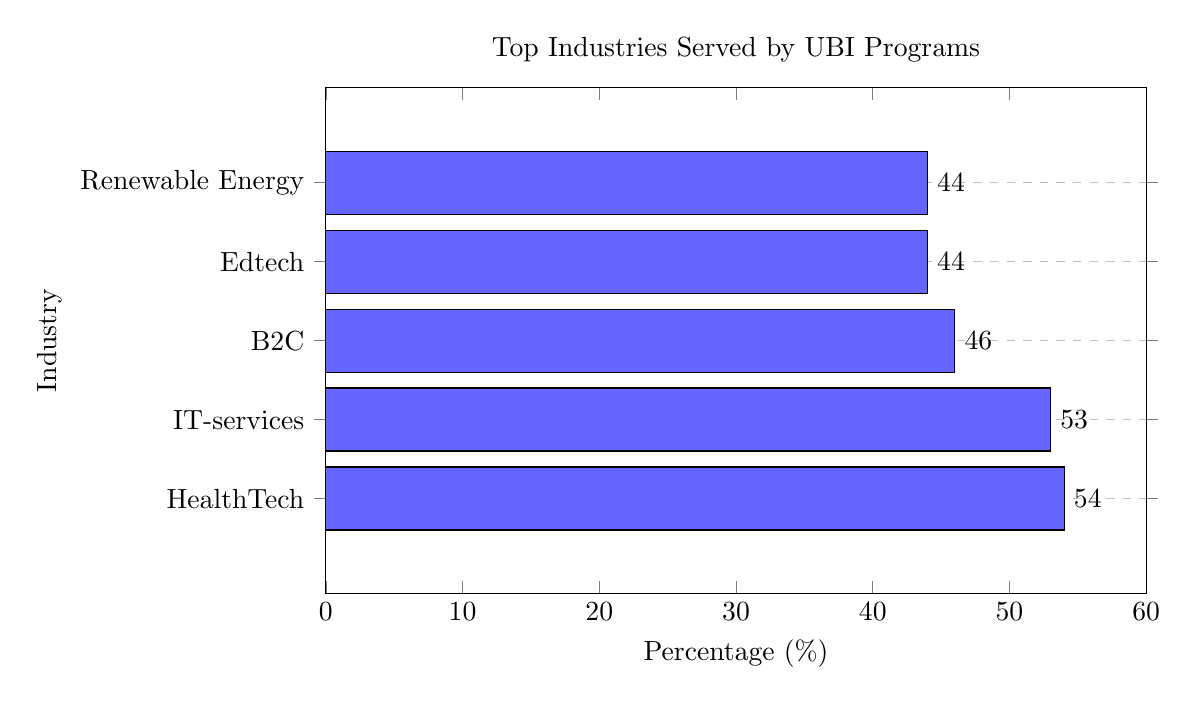
\begin{tikzpicture}
			\begin{axis}[
				title={Top Industries Served by UBI Programs},
				xlabel={Percentage (\%)},
				ylabel={Industry},
				xbar,
				xmin=0,
				xmax=60,
				width=12cm,
				height=8cm,
				bar width=0.8cm,
				nodes near coords,
				nodes near coords align={horizontal},
				ytick=data,
				yticklabels={HealthTech, IT-services, B2C, Edtech, Renewable Energy},
				ymajorgrids=true,
				grid style=dashed,
				enlarge y limits=0.3
			]
			\addplot[fill=blue!60] coordinates {
				(54,0)
				(53,1)
				(46,2)
				(44,3)
				(44,4)
			};
			\end{axis}
		\end{tikzpicture}
		\caption{Distribution of top industries served by UBI programs globally (Source: UBI Global Community Report 2023)}
		\label{fig:top_industries}
	\end{figure}

	\begin{figure}[h]
		\centering
		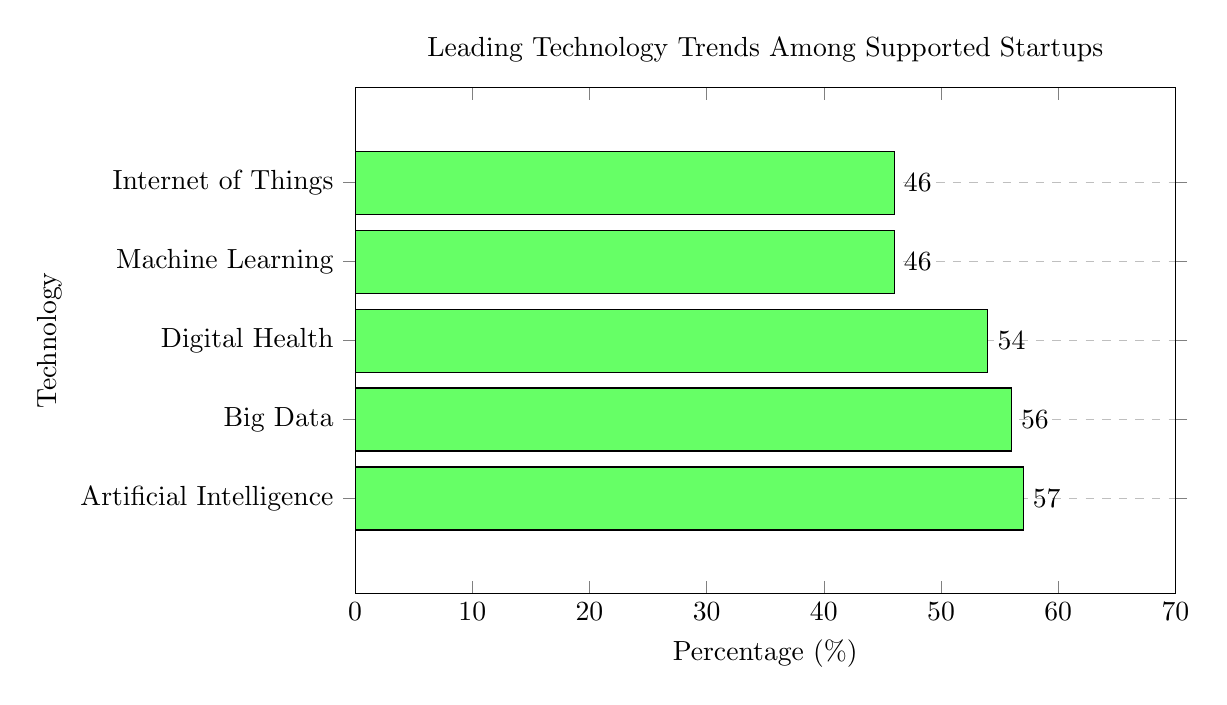
\begin{tikzpicture}
			\begin{axis}[
				title={Leading Technology Trends Among Supported Startups},
				xlabel={Percentage (\%)},
				ylabel={Technology},
				xbar,
				xmin=0,
				xmax=70,
				width=12cm,
				height=8cm,
				bar width=0.8cm,
				nodes near coords,
				nodes near coords align={horizontal},
				ytick=data,
				yticklabels={Artificial Intelligence, Big Data, Digital Health, Machine Learning, Internet of Things},
				ymajorgrids=true,
				grid style=dashed,
				enlarge y limits=0.3
			]
			\addplot[fill=green!60] coordinates {
				(57,0)
				(56,1)
				(54,2)
				(46,3)
				(46,4)
			};
			\end{axis}
		\end{tikzpicture}
		\caption{Distribution of leading technology trends among startups supported by UBI programs (Source: UBI Global Community Report 2023)}
		\label{fig:technology_trends}
	\end{figure}

	\begin{figure}[h]
		\centering
		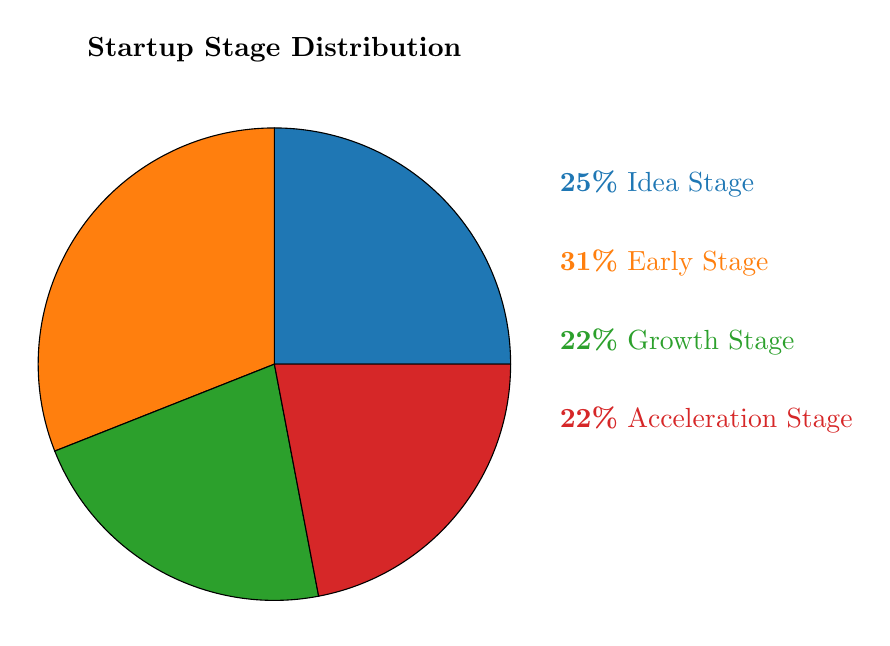
\begin{tikzpicture}
			% Define colors
			\definecolor{color1}{RGB}{31,119,180}
			\definecolor{color2}{RGB}{255,127,14}
			\definecolor{color3}{RGB}{44,160,44}
			\definecolor{color4}{RGB}{214,39,40}
			
			% Data
			\def\idea{25}
			\def\early{31}
			\def\growth{22}
			\def\accel{22}

			% Pre-calculate angles
			\pgfmathsetmacro{\angleA}{\idea*3.6}
			\pgfmathsetmacro{\angleB}{(\idea+\early)*3.6}
			\pgfmathsetmacro{\angleC}{(\idea+\early+\growth)*3.6}
			
			% Draw pie slices
			\draw[fill=color1] (0,0) -- (0:3) arc (0:\angleA:3) -- cycle;
			\draw[fill=color2] (0,0) -- (\angleA:3) arc (\angleA:\angleB:3) -- cycle;
			\draw[fill=color3] (0,0) -- (\angleB:3) arc (\angleB:\angleC:3) -- cycle;
			\draw[fill=color4] (0,0) -- (\angleC:3) arc (\angleC:360:3) -- cycle;
			
			% Add labels
			\node at (0,4) {\textbf{Startup Stage Distribution}};
			\node[above right] at (3.5,2) {\textcolor{color1}{\textbf{25\%} Idea Stage}};
			\node[above right] at (3.5,1) {\textcolor{color2}{\textbf{31\%} Early Stage}};
			\node[above right] at (3.5,0) {\textcolor{color3}{\textbf{22\%} Growth Stage}};
			\node[above right] at (3.5,-1) {\textcolor{color4}{\textbf{22\%} Acceleration Stage}};
		\end{tikzpicture}
		\caption{Distribution of startup stages supported by UBI programs (Source: UBI Global Community Report 2023)}
		\label{fig:startup_stages}
	\end{figure}

	\textbf{Change Tendency (2019-2020 to 2021-2022 and 2023):}
	From 2019-2020 to 2021-2022, UBI Global's benchmark studies show a significant reduction in the number of programs and countries included in the formal benchmarking process, with assessed programs dropping from 364 to 109 and countries from 82 to 56. This likely reflects a more stringent selection process, a focus on top-tier programs, or changes in participation rates. Despite this, the 2023 UBI Global Community report demonstrates that the broader global network of business incubators and accelerators remains extensive, with over 1,000 programs in 90+ countries. The 2023 data also highlights the increasing diversity of program types, sector focus, and regional participation, as well as the continued dominance of university-based incubators. This evolution suggests that while formal benchmarking has become more selective, the overall ecosystem is expanding and diversifying, adapting to new trends and regional needs.
	
	\begin{figure}[h]
		\centering
		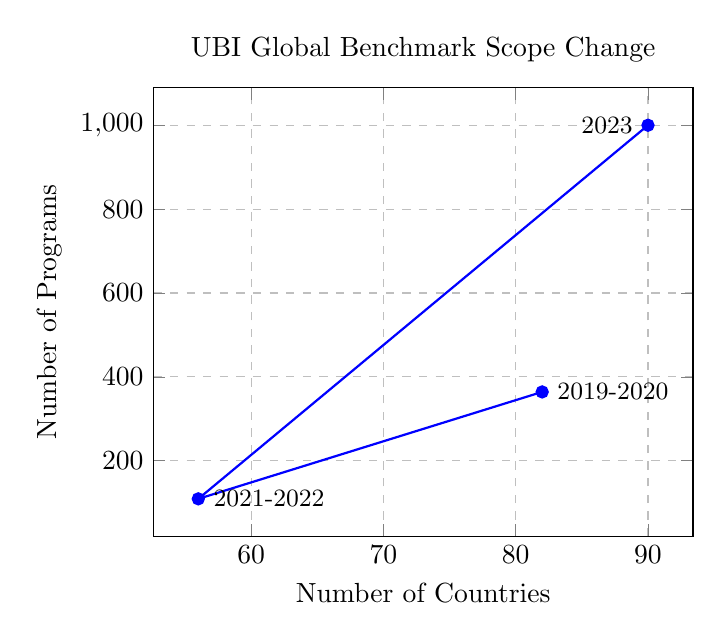
\begin{tikzpicture}
			\begin{axis}[
				title={UBI Global Benchmark Scope Change},
				xlabel={Number of Countries},
				ylabel={Number of Programs},
				ymajorgrids=true,
				xmajorgrids=true,
				grid style=dashed
			]
			
			% Add the plot with a connecting line
			\addplot[color=blue, mark=*, thick] coordinates {
				(82,364) 
				(56,109)
				(90,1000)
			};
			
			% Add labels to the points using relative positioning
			\node[right, font=\small, xshift=2pt] at (axis cs:82,364) {2019-2020};
			\node[right, font=\small, xshift=2pt] at (axis cs:56,109) {2021-2022};
			\node[left, font=\small, xshift=-2pt] at (axis cs:90,1000) {2023};
			
			\end{axis}
		\end{tikzpicture}
		\caption{Change in scope of UBI Global's benchmark studies, plotting programs vs. countries for the 2019-2020, 2021-2022, and 2023 periods.}
		\label{fig:ubi_change_tendency}
	\end{figure}
	
	\subsection{Key Performance Indicators (KPIs) and Impact Measurement Framework}
	UBI Global's comprehensive methodology for assessing program impact and performance consistently utilizes \textbf{21 Key Performance Indicators (KPIs)} across both the 2019-2020 and 2021-2022 benchmark studies \autocite{ubi2019world, ubi2021world}. These KPIs are systematically grouped into three main categories, each contributing to a Program Impact and Performance Score (PIPS). All fiscal information is standardized to 2018 US dollars in the 2019-2020 report and likely similar in the 2021-2022 report for consistency.

	\begin{itemize}
		\item \textbf{Value for Ecosystem (33.3\% weight of PIPS)}: This category assesses the economic impact of the programs and their client/alumni startups, as well as their success in retaining human capital and ventures within the innovation ecosystem. It includes subcategories like "Economy Enhancement" and "Talent Retention" \autocite{ubi2019world, ubi2021world}.
		\begin{itemize}
			\item \textit{Economy Enhancement} (22.2\% of PIPS) measures: Jobs created \& sustained, Sales revenue, Graduates (within 5 years), and Self-generated revenue.
			\item \textit{Talent Retention} (11.1\% of PIPS) measures: Client startups accepted (within 1 year) and Graduate retention (within 5 years).
		\end{itemize}
		\item \textbf{Value for Client Startups (33.3\% weight of PIPS)}: This category evaluates the quantity and efficiency of services provided by the programs, alongside their critical function as facilitators of community and network building. It comprises subcategories such as "Competence Development," "Access to Funds," and "Access to Network" \autocite{ubi2019world, ubi2021world}.
		\begin{itemize}
			\item \textit{Competence Development} (8.9\% of PIPS) measures: Services offered and Coaching \& mentoring hours.
			\item \textit{Access to Funds} (11.1\% of PIPS) measures: Total investment attracted (within 5 years), Average investment attracted (within 5 years), and Seed funding attraction (within 1 year).
			\item \textit{Access to Network} (13.3\% of PIPS) measures: Partners, Events, and Alumni engagement.
		\end{itemize}
		\item \textbf{Value for Program (33.3\% weight of PIPS)}: This category assesses the program's success in attracting deal flow and third-party support, as well as its capacity to foster the creation of viable companies. It includes "Program Attractiveness" and "Post-Graduation Performance" subcategories \autocite{ubi2019world, ubi2021world}.
		\begin{itemize}
			\item \textit{Program Attractiveness} (15.5\% of PIPS) measures: In-state applications, Out-of-state applications, and Sponsorship attraction.
			\item \textit{Post-Graduation Performance} (17.8\% of PIPS) measures: 1-year survival rate (within 10 years), 5-year survival rate (within 10 years), High-growth enterprises (within 10 years), and Qualified exits (within 10 years).
		\end{itemize}
	\end{itemize}
	While these reports detail the comprehensive KPIs utilized for benchmarking and ranking, they focus on the comparative performance of individual programs rather than providing aggregate global numerical data for the entire sample's performance across all these metrics.
	
	\subsection{Leading University Business Incubators Globally}
	UBI Global's World Rankings consistently recognize top-performing university business incubators based on their outstanding impact and value creation. The following tables show a sample of these leading incubators for the two benchmark periods.

	\begin{table}[H]
		\centering
		\caption{Leading University Business Incubators (2019-2020 Sample) \autocite{ubi2019world}}
		\label{tab:leading_ubis_2019}
		\resizebox{\textwidth}{!}{%
		\begin{tabular}{|l|l|l|}
			\hline
			\textbf{Incubator} & \textbf{University} & \textbf{Country} \\
			\hline
			Chalmers Ventures & Chalmers University of Technology & Sweden \\
			The DMZ at Ryerson University & Ryerson University & Canada \\
			IPN Incubadora & University of Coimbra, Polytechnic Institute of Coimbra & Portugal \\
			PoliHub - Innovation District \& Startup Accelerator & Politecnico di Milano & Italy \\
			The SETsquared Partnership & Univ. of Bath, Bristol, Exeter, Southampton, Surrey & UK \\
			University of Toronto Entrepreneurship & University of Toronto & Canada \\
			UtrechtInc & Utrecht University, Medical Center Utrecht, UAS Utrecht & Netherlands \\
			YES!Delft & Delft University of Technology, The Hague UAS & Netherlands \\
			\hline
		\end{tabular}%
		}
	\end{table}

	\begin{table}[H]
		\centering
		\caption{Leading University Business Incubators (2021-2022 Sample) \autocite{ubi2021world}}
		\label{tab:leading_ubis_2021}
		\resizebox{\textwidth}{!}{%
		\begin{tabular}{|l|l|l|}
			\hline
			\textbf{Incubator} & \textbf{University} & \textbf{Country} \\
			\hline
			Center for Technology Development (CDT) & University of Brasilia & Brazil \\
			CEI UCN & Universidad Catolica del Norte & Chile \\
			EUREKA & University of Chile & Chile \\
			Innovation, Business, and Economy Center (CIE) & Autonomous University of Baja California & Mexico \\
			King Abdullah University of Science and Technology & King Abdullah University of Science and Technology & Saudi Arabia \\
			MCB & Federal University of Campina Grande & Brazil \\
			The DMZ at Toronto Metropolitan University & Toronto Metropolitan University & Canada \\
			University of Toronto Entrepreneurship & University of Toronto & Canada \\
			UtrechtInc & Utrecht Univ., Medical Center Utrecht, UAS Utrecht, HKU Arts & Netherlands \\
			\hline
		\end{tabular}%
		}
	\end{table}
	
	These examples illustrate the continued global reach and diverse institutional affiliations of leading UBIs across different reporting periods.

	\section{Vietnam UBIs Quantitative Data}
	The Vietnamese landscape for university-based incubation programs (UBIs) and the broader startup ecosystem has undergone substantial development, marked by increasing governmental support, robust private sector engagement, and a growing entrepreneurial culture.

	\subsection{Evolution of the Startup Ecosystem and University Engagement}
	The foundational elements of Vietnam's startup ecosystem were solidified in the mid-2010s. A pivotal initiative was the Prime Minister's approval of the "National Program to Support Innovative Startup Ecosystem in Vietnam by the Year 2025," coupled with the designation of 2016 as the "Nation Year of Startup" \autocite{dinh2017promoting}. This period witnessed a notable rise in entrepreneurial awareness, with the Vietnam Startup Index Report 2015/2016 indicating that the proportion of adults cognizant of business opportunities increased from 36.8\% in 2013 to 56.8\% in 2015, positioning Vietnam 9th among 60 surveyed countries \autocite{dinh2017promoting}. Early university involvement manifested through the establishment of spin-off companies and business incubators. By September 2016, Vietnam operated 12 business incubators, evenly distributed between the northern (5) and southern (7) regions \autocite{dinh2017promoting}. Pioneering university spin-offs, such as BK-Holdings (Hanoi University of Science and Technology) and TOPICA Education Technology Association, demonstrated the early potential of academic entrepreneurship \autocite{dinh2017promoting}. These university-led ventures were crucial in fostering university-enterprise linkages and technology transfer, as exemplified by Vietnam National University's (VNU) Natural Sciences Company, which executed over 90 technology transfer contracts from 2011 to 2015 \autocite{dinh2017promoting}. An internal survey in 2015 revealed that over 80\% of IT students in Ho Chi Minh City expressed a desire to initiate businesses during their studies, signaling a strong entrepreneurial inclination within the student body \autocite{dinh2017promoting}.

	\begin{figure}
		\centering
		\begin{tikzpicture}
		\begin{axis}[
			xbar stacked,
			width=15cm,
			height=8cm,
			bar width=18pt,
			xmin=0, xmax=100,
			ytick=data,
			yticklabels={2023,2022,2021,2020,2019,2018,2017},
			xlabel={\%},
			legend style={at={(0.5,-0.18)}, anchor=north, legend columns=6, font=\small},
			xtick={0,20,40,60,80,100},
			tick label style={font=\small},
			ylabel={},
			title={Proportion of investment value by country},
			title style={yshift=1.5em, font=\bfseries\large},
			enlarge y limits=0.15,
			point meta=explicit,
			nodes near coords={\pgfmathprintnumber[assume math mode=true]{\pgfplotspointmeta}\%},
			nodes near coords align={center},
			nodes near coords style={font=\small, color=white,
				/pgf/number format/precision=0,
				/pgf/number format/fixed,
				/pgf/number format/fixed zerofill=false
			},
			]
		% Indonesia
		\addplot+[xbar, fill=gray!60, draw=none] coordinates {(23,0) [23] (44,1) [44] (41,2) [41] (67,3) [67] (52,4) [52] (67,5) [67] (65,6) [65]};
		% Singapore
		\addplot+[xbar, fill=gray!40, draw=none] coordinates {(56,0) [56] (27,1) [27] (33,2) [33] (14,3) [14] (19,4) [19] (0,5) [0] (19,6) [19]};
		% Malaysia
		\addplot+[xbar, fill=gray!30, draw=none] coordinates {(3,0) [3] (6,1) [6] (4,2) [4] (3,3) [3] (3,4) [3] (18,5) [18] (3,6) [3]};
		% Thailand
		\addplot+[xbar, fill=gray!20, draw=none] coordinates {(2,0) [2] (6,1) [6] (3,2) [3] (6,3) [6] (3,4) [3] (3,5) [3] (8,6) [8]};
		% Philippines
		\addplot+[xbar, fill=gray!10, draw=none] coordinates {(6,0) [6] (9,1) [9] (6,2) [6] (2,3) [2] (0,4) [0] (2,5) [2] (2,6) [2]};
		% Vietnam
		\addplot+[xbar, fill=vncolor, draw=none] coordinates {(9,0) [9] (8,1) [8] (13,2) [13] (8,3) [8] (23,4) [23] (9,5) [9] (2,6) [2]};
		\legend{Indonesia, Singapore, Malaysia, Thailand, Philippines, Vietnam}
		\end{axis}
		\end{tikzpicture}
		\caption{Proportion of investment value by country (2017--2023) \autocite{vietnam_innovation_report_2024}.}
		\end{figure}
		
		\vspace{1cm}
		
		\begin{figure}
		\centering
		\begin{tikzpicture}
		\begin{axis}[
			xbar stacked,
			width=15cm,
			height=8cm,
			bar width=18pt,
			xmin=0, xmax=100,
			ytick=data,
			yticklabels={2023,2022,2021,2020,2019,2018,2017},
			xlabel={\%},
			legend style={at={(0.5,-0.18)}, anchor=north, legend columns=6, font=\small},
			xtick={0,20,40,60,80,100},
			tick label style={font=\small},
			ylabel={},
			title={Proportion of investment deals by country},
			title style={yshift=1.5em, font=\bfseries\large},
			enlarge y limits=0.15,
			point meta=explicit,
			nodes near coords={\pgfmathprintnumber[assume math mode=true]{\pgfplotspointmeta}\%},
			nodes near coords align={center},
			nodes near coords style={font=\small, color=white,
				/pgf/number format/precision=0,
				/pgf/number format/fixed,
				/pgf/number format/fixed zerofill=false
			},
			]
		% Indonesia
		\addplot+[xbar, fill=gray!60, draw=none] coordinates {(18,0) [18] (26,1) [26] (24,2) [24] (26,3) [26] (23,4) [23] (30,5) [30] (30,6) [30]};
		% Singapore
		\addplot+[xbar, fill=gray!40, draw=none] coordinates {(52,0) [52] (39,1) [39] (40,2) [40] (36,3) [36] (34,4) [34] (32,5) [32] (34,6) [34]};
		% Malaysia
		\addplot+[xbar, fill=gray!30, draw=none] coordinates {(6,0) [6] (9,1) [9] (8,2) [8] (11,3) [11] (10,4) [10] (11,5) [11] (13,6) [13]};
		% Thailand
		\addplot+[xbar, fill=gray!20, draw=none] coordinates {(3,0) [3] (4,1) [4] (4,2) [4] (5,3) [5] (9,4) [9] (8,5) [8] (10,6) [10]};
		% Philippines
		\addplot+[xbar, fill=gray!10, draw=none] coordinates {(8,0) [8] (5,1) [5] (5,2) [5] (5,3) [5] (4,4) [4] (4,5) [4] (6,6) [6]};
		% Vietnam
		\addplot+[xbar, fill=vncolor, draw=none] coordinates {(12,0) [12] (16,1) [16] (19,2) [19] (17,3) [17] (20,4) [20] (16,5) [16] (8,6) [8]};
		\legend{Indonesia, Singapore, Malaysia, Thailand, Philippines, Vietnam}
		\end{axis}
		\end{tikzpicture}
		\caption{Proportion of investment deals by country (2017--2023) \autocite{vietnam_innovation_report_2024}.}
	\end{figure}

Vietnam maintains its third position in Southeast Asia in terms of deal count and returns to the third position in investment value. Singapore leads in both investment value and deal count, followed by Indonesia.

	Post-2017, the ecosystem experienced accelerated growth. The government's continued commitment is evident in initiatives like Project 844, launched in 2016 and expanded in 2021 (Decision No. 188/QD-TTg), which has extended its support to 60 provinces by 2024, with 40 localities developing financial mechanisms for startups \autocite{nssc2024project}. Furthermore, Decree No. 109/2022/ND-CP specifically targets the fostering of the innovative startup ecosystem within universities \autocite{nssc2024project}. The establishment of the National Innovation Center (NIC) in 2023 at Hoa Lac Hi-Tech Park serves as a central hub for promoting sustainable growth driven by science, technology, and innovation \autocite{vietnam_innovation_report_2024}. By the end of 2024, Vietnam's startup ecosystem comprised over \textbf{4,000 startups}, including two unicorn companies and eleven valued over \$100 million.

	\subsection{Investment Trends and Global Standing}
	Vietnam's position in the global innovation landscape has steadily strengthened. In the Global Innovation Index 2023, Vietnam ascended to \textbf{46th position} out of 132 countries, demonstrating consistent improvement \autocite{vietnam_innovation_report_2024}. The country is also recognized among the top 7 middle-income economies with the most significant innovation progress over the past decade \autocite{vietnam_innovation_report_2024}. According to StartupBlink's Global Startup Ecosystem Index 2024, Vietnam rose to \textbf{56th globally} (from 58th in 2023), securing 5th place in Southeast Asia and 12th in Asia-Pacific \autocite{startupblink2024, vietnamnews2024pm}.

	The venture capital landscape, while subject to global fluctuations, exhibited resilience in Vietnam. In 2023, Vietnamese startups attracted a total investment of \textbf{\$529 million} \autocite{vietnam_innovation_report_2024}. This represented a 17\% decline compared to the previous year, yet it was notably milder than the 35\% global venture capital investment contraction, indicating the market's intrinsic strength \autocite{vietnam_innovation_report_2024}. Vietnam maintained its third position in Southeast Asia for the volume of investment deals and successfully reclaimed the third position in total investment value within the region, trailing only Singapore and Indonesia \autocite{vietnam_innovation_report_2024}.

	\begin{figure}[H]
		\centering
		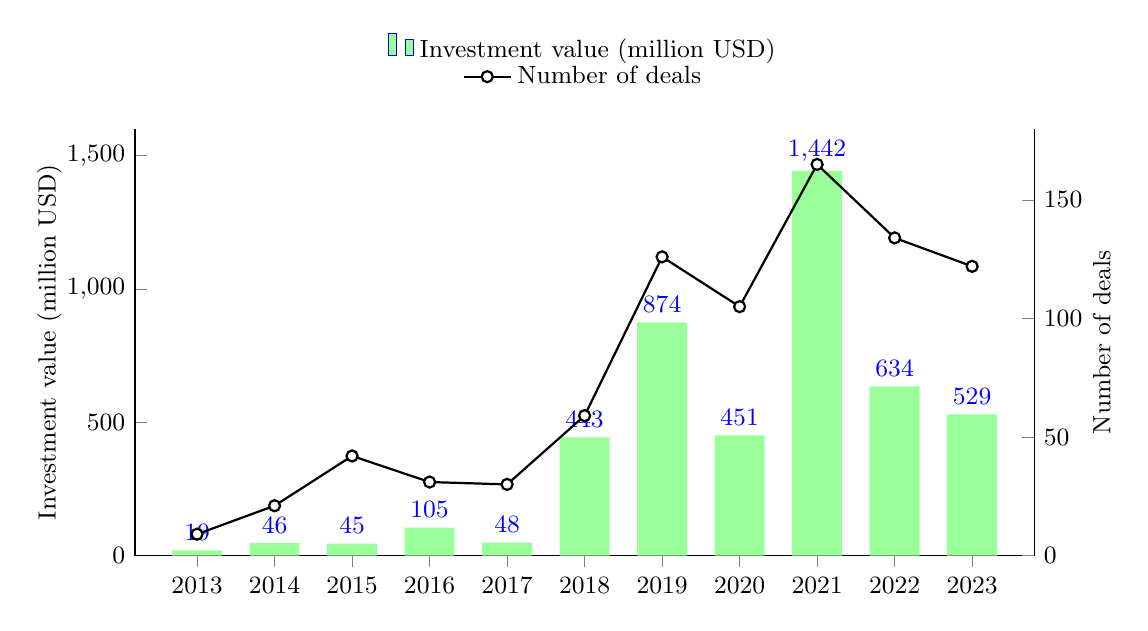
\begin{tikzpicture}
			\begin{axis}[
				width=13cm,
				height=7cm,
				ybar,
				bar width=18pt,
				ymin=0,
				ymax=1600,
				ylabel={Investment value (million USD)},
				ylabel style={yshift=-0.5em},
				axis y line*=left,
				axis x line*=bottom,
				symbolic x coords={2013,2014,2015,2016,2017,2018,2019,2020,2021,2022,2023},
				xtick=data,
				enlarge x limits=0.08,
				nodes near coords,
				nodes near coords style={above, font=\small, color=blue, text opacity=1, fill opacity=1, draw opacity=1},
				nodes near coords align={vertical},
				tick label style={font=\small},
				label style={font=\small},
				legend style={at={(0.5,1.13)}, anchor=south, legend columns=-1, font=\small, draw=none, fill=none},
			]
			% Bar plot: Investment value
			\addplot+[ybar, fill=green!40!white, draw=none] coordinates {
				(2013, 19)
				(2014, 46)
				(2015, 45)
				(2016, 105)
				(2017, 48)
				(2018, 443)
				(2019, 874)
				(2020, 451)
				(2021, 1442)
				(2022, 634)
				(2023, 529)
			};
			\addlegendentry{Investment value (million USD)}
			\end{axis}

			% Overlay line plot for number of deals
			\begin{axis}[
				width=13cm,
				height=7cm,
				ymin=0,
				ymax=180,
				axis y line*=right,
				axis x line=none,
				ylabel={Number of deals},
				ylabel style={yshift=0.3em},
				symbolic x coords={2013,2014,2015,2016,2017,2018,2019,2020,2021,2022,2023},
				xtick=data,
				enlarge x limits=0.08,
				legend style={at={(0.5,1.07)}, anchor=south, legend columns=-1, font=\small, draw=none, fill=none},
				every node near coord/.append style={font=\small, yshift=-10pt, color=black},
				tick label style={font=\small},
				label style={font=\small},
			]
			% Line plot: Number of deals
			\addplot+[
				mark=*,
				mark options={fill=white},
				color=black,
				thick
			] coordinates {
				(2013, 9)
				(2014, 21)
				(2015, 42)
				(2016, 31)
				(2017, 30)
				(2018, 59)
				(2019, 126)
				(2020, 105)
				(2021, 165)
				(2022, 134)
				(2023, 122)
			};
			\addlegendentry{Number of deals}
			\end{axis}
		\end{tikzpicture}
		\caption{Investment value and number of startup deals in Vietnam (2013--2023) \autocite{vietnam_innovation_report_2024}.}
		\label{fig:vn-startup-investment}
	\end{figure}

	Sectoral investment patterns in 2023 revealed significant shifts:
	\begin{itemize}
	\item The Healthcare sector experienced a record-high investment, surging by 391\% year-over-year to become the leading invested sector \autocite{vietnam_innovation_report_2024}.
	\item The Education sector also reached its highest-ever investment volume, increasing by 107\% year-over-year \autocite{vietnam_innovation_report_2024}.
	\end{itemize}
	Approximately 100 funds contributed capital to Vietnamese startups in 2023, with Singaporean investors being the most active, closely followed by domestic Vietnamese investors \autocite{vietnam_innovation_report_2024}. The exit market for startups is also evolving positively, marked by growth in the public market, refined stock market regulatory mechanisms, and an increasing role of local corporations in mergers and acquisitions \autocite{vietnam_innovation_report_2024}.

	Despite remarkable progress, the Vietnamese university startup ecosystem continues to face challenges. These include a persistent gap between theoretical instruction and practical application in training programs, which limits hands-on experience \autocite{nhandan2025startup}. Universities frequently contend with insufficient financial resources, inadequate infrastructure, and a dearth of experimental spaces and early-stage investment funds \autocite{nhandan2025startup}. Furthermore, attracting international resources and securing foreign investment remains challenging, partly due to complexities in corporate restructuring requirements (e.g., establishing an offshore parent company) and regulatory ambiguities \autocite{bssc2025wave, nssc2024challenges}. Startups also contend with a scarcity of suitable strategic advisors and disparities in resource access between urban and rural areas \autocite{ueh2024vc}. The Prime Minister has emphasized the need for a stronger ecosystem, urging enhanced policies, particularly in finance and intellectual property, and promoting public-private partnerships to establish student startup support funds \autocite{vietnamnews2025pm}.

	\section{Research Methodology and Data Collection}
	
	\subsection{Research Design and Approach}
	This study employs a mixed-methods research approach, combining quantitative survey data with qualitative interview insights to comprehensively examine the impact of University-Based Incubation Programs (UBIs) on startup performance in Vietnam. The research design follows a sequential explanatory strategy, where quantitative data collection precedes qualitative data gathering to provide deeper contextual understanding of the statistical findings.
	
	The quantitative component utilizes a cross-sectional survey design to collect data from startup founders and key personnel who have participated in UBI programs. This approach enables the measurement of multiple variables simultaneously and facilitates the application of Structural Equation Modeling (SEM) to test the hypothesized relationships between UBI resources, innovation capacity, and startup performance.
	
	The qualitative component involves semi-structured interviews with UBI program managers, mentors, and selected startup founders to gain deeper insights into the mechanisms through which UBI resources influence startup outcomes. This triangulation approach enhances the validity and reliability of the research findings by corroborating quantitative results with qualitative evidence.
	
	\subsection{Target Population and Sampling Strategy}
	The target population for this study comprises startup founders and key personnel from Vietnamese startups that have participated in University-Based Incubation Programs. The sampling frame includes startups affiliated with major UBI programs in Vietnam, specifically:
	
	\begin{itemize}
		\item Hanoi University of Science and Technology (HUST) - BK-Holdings
		\item University of Danang - Innovation and Incubation Center
		\item National University of Ho Chi Minh City (VNU-HCM) - Technology Incubation Center
		\item Other university-based incubation programs across Vietnam
	\end{itemize}
	
	A purposive sampling strategy was employed to ensure representation across different startup stages, industries, and geographic regions. The inclusion criteria for participation were:
	\begin{itemize}
		\item Startups must have been established within the last 10 years
		\item Active participation in a UBI program for at least 6 months
		\item Availability of key performance metrics (revenue, growth, market penetration)
		\item Willingness to provide detailed information about their UBI experience
	\end{itemize}
	
	The sample size determination followed the guidelines for SEM analysis, which recommends a minimum of 10-15 observations per parameter estimate. Given the complexity of the proposed model with multiple latent variables and path relationships, a target sample size of 200-250 startups was established to ensure adequate statistical power and model stability.
	
	\subsection{Data Collection Instruments}
	
	\subsubsection{Survey Questionnaire Design}
	The primary data collection instrument was a comprehensive survey questionnaire designed to capture detailed information about startup characteristics, UBI program engagement, resource utilization, and performance outcomes. The questionnaire was developed based on extensive literature review and pilot testing with a small group of startup founders to ensure clarity and relevance.
	
	The survey instrument consists of six main sections:
	
	\textbf{Part 1: Startup Information}
	This section collects basic demographic and descriptive information about the participating startups, including:
	\begin{itemize}
		\item Startup name and year of establishment
		\item Industry classification (Technology, HealthTech, Renewable Energy, FinTech, or Other)
		\item Current stage of development (Idea, Early, Growth, or Acceleration Stage)
	\end{itemize}
	
	\textbf{Part 2: UBI Program Engagement}
	This section examines the nature and extent of startup involvement with UBI programs:
	\begin{itemize}
		\item Specific UBI program affiliation
		\item Duration of participation (Less than 6 months, 6-12 months, 1-2 years, Over 2 years)
		\item Types of support received (Mentorship, Funding, Networking, Training, Infrastructure, Others)
	\end{itemize}
	
	\textbf{Part 3: UBI Resource Evaluation}
	This section employs a 5-point Likert scale (1 = Very Ineffective to 5 = Very Effective) to assess the perceived effectiveness of different UBI resources:
	\begin{itemize}
		\item \textbf{Mentorship}: Strategic direction guidance, industry connections, challenge resolution
		\item \textbf{Funding}: Financial stability contribution, scaling resources, investment attraction
		\item \textbf{Networking}: Partnership establishment, stakeholder access, market penetration
		\item \textbf{Training and Workshops}: Growth relevance, skill enhancement, trend awareness
		\item \textbf{Infrastructure/Workspace}: Operational efficiency, product development acceleration
	\end{itemize}
	
	\textbf{Part 4: Innovation Capacity and Startup Performance}
	This section measures key outcome variables:
	\begin{itemize}
		\item Innovation capacity rating (Very low to Very high)
		\item Performance metrics: Revenue growth percentage, new products launched, market penetration
		\item UBI program impact assessment on market penetration and overall success
	\end{itemize}
	
	\textbf{Part 5: Suggestions for UBI Program Improvement}
	This section captures recommendations for program enhancement and willingness to recommend the program to others.
	
	\textbf{Part 6: Additional Comments}
	An open-ended section for qualitative feedback and suggestions.
	
	\begin{longtable}{|p{4cm}|p{8cm}|p{3cm}|}
	\caption{The survey questionnaire}\\
	\hline
	\textbf{Characteristics} & \textbf{Distribution} & \textbf{Author(s)} \\
	\hline
	\endfirsthead
	\caption[]{The survey questionnaire (continued)}\\
	\hline
	\textbf{Characteristics} & \textbf{Distribution} & \textbf{Author(s)} \\
	\hline
	\endhead
	\hline
	\multicolumn{3}{r}{\textit{Continued on next page}} \\
	\endfoot
	\hline
	\endlastfoot
	\multicolumn{3}{|c|}{\textbf{Part 1: Startup Information}} \\
	\hline
	Startup Name & Open text & Mamakou and Manaras (2014) \\
	\cline{1-2}
	Year of Establishment & Open text & \\
	\cline{1-2}
	Industry & Technology, HealthTech, Renewable Energy, FinTech, Other (specify) & \\
	\cline{1-2}
	Current Stage & Idea Stage, Early Stage, Growth Stage, Acceleration Stage & \\
	\hline
	\multicolumn{3}{|c|}{\textbf{Part 2: UBI Engagement}} \\
	\hline
	UBI Program Affiliation & HUST, University of Danang, National University of HCMC, Other (specify) & \\
	\cline{1-2}
	Duration in UBI Program & Less than 6 months, 6-12 months, 1-2 years, Over 2 years & \\
	\cline{1-2}
	Types of Support Received & Mentorship, Funding, Networking, Training/Workshops, Infrastructure/Workspace, Other (specify) & \\
	\hline
	\multicolumn{3}{|c|}{\textbf{Part 3: UBI Resource Evaluation (1--5 scale)}} \\
	\hline
	Mentorship & 3 statements, each rated 1 (Very Ineffective) to 5 (Very Effective) & \\
	\cline{1-2}
	Funding & 3 statements, each rated 1 (Very Ineffective) to 5 (Very Effective) & \\
	\cline{1-2}
	Networking Opportunities & 3 statements, each rated 1 (Very Ineffective) to 5 (Very Effective) & \\
	\cline{1-2}
	Training and Workshops & 3 statements, each rated 1 (Very Ineffective) to 5 (Very Effective) & \\
	\cline{1-2}
	Infrastructure/Workspace & 2 statements, each rated 1 (Very Ineffective) to 5 (Very Effective) & \\
	\hline
	\multicolumn{3}{|c|}{\textbf{Part 4: Innovation Capacity and Startup Performance}} \\
	\hline
	Startup Innovation Capacity & Very low, Low, Moderate, High, Very high & \\
	\cline{1-2}
	Revenue Growth (\%) & Open text & \\
	\cline{1-2}
	Number of New Products Launched & Open text & \\
	\cline{1-2}
	Market Penetration (new customers) & 1-20\%, 21-50\%, 51-100\%, Over 100\% & \\
	\cline{1-2}
	UBI Impact on Market Penetration & Yes, significantly; Yes, moderately; No, not at all & \\
	\cline{1-2}
	Overall UBI Impact & Very negative, Negative, Neutral, Positive, Very positive & \\
	\hline
	\multicolumn{3}{|c|}{\textbf{Part 5: Suggestions for UBI Program Improvement}} \\
	\hline
	Additional Support Desired & More mentorship, More funding, Improved networking, Additional training (specify), Other (specify) & \\
	\cline{1-2}
	Recommend UBI Program? & Yes, No, Maybe & \\
	\hline
	\multicolumn{3}{|c|}{\textbf{Part 6: Additional Comments}} \\
	\hline
	Other Comments/Feedback & Open text & \\
	\hline
	\end{longtable}

	\subsubsection{Complete Survey Questionnaire}
	The following is the complete survey questionnaire used for data collection:
	
	\begin{center}
	\textbf{SURVEY ON THE IMPACT OF UNIVERSITY-BASED INCUBATION PROGRAMS ON STARTUP PERFORMANCE}
	\end{center}
	
	\textbf{Part 1: Startup Information}
	\begin{itemize}
		\item \textbf{Startup Name:} \underline{\hspace{4cm}}
		\item \textbf{Year of Establishment:} \underline{\hspace{4cm}}
		\item \textbf{Industry (Select one):}
		\begin{itemize}
			\item Technology (Tech)
			\item HealthTech
			\item Renewable Energy
			\item FinTech
			\item Other (Please specify): \underline{\hspace{4cm}}
		\end{itemize}
		\item \textbf{Current Stage of the Startup (Select one):}
		\begin{itemize}
			\item Idea Stage
			\item Early Stage
			\item Growth Stage
			\item Acceleration Stage
		\end{itemize}
	\end{itemize}
	
	\textbf{Part 2: University-Based Incubation Program (UBI) Engagement}
	\begin{itemize}
		\item \textbf{Which University-Based Incubation Program are you affiliated with?}
		\begin{itemize}
			\item Hanoi University of Science and Technology
			\item University of Danang
			\item National University of Ho Chi Minh City
			\item Other (Please specify): \underline{\hspace{4cm}}
		\end{itemize}
		\item \textbf{How long have you been participating in the UBI program?}
		\begin{itemize}
			\item Less than 6 months
			\item 6-12 months
			\item 1-2 years
			\item Over 2 years
		\end{itemize}
		\item \textbf{Which types of support have you received from the UBI program? (Select all that apply):}
		\begin{itemize}
			\item Mentorship
			\item Funding
			\item Networking Opportunities
			\item Training and Workshops
			\item Infrastructure/Workspace
			\item Others (Please specify): \underline{\hspace{4cm}}
		\end{itemize}
	\end{itemize}
	
	\textbf{Part 3: UBI Resource Evaluation}
	\textbf{Please rate the following statements about each UBI resource on a scale from 1 (Very Ineffective) to 5 (Very Effective):}
	
	\textbf{Mentorship}
	\begin{itemize}
		\item The mentorship I received from the UBI program was beneficial in shaping the strategic direction of my startup.
		\begin{center}
		\begin{tabular}{cccccc}
		1 & 2 & 3 & 4 & 5 \\
		Very Ineffective & & & & Very Effective
		\end{tabular}
		\end{center}
		\item The mentors provided valuable industry connections that helped my startup grow.
		\begin{center}
		\begin{tabular}{cccccc}
		1 & 2 & 3 & 4 & 5 \\
		Very Ineffective & & & & Very Effective
		\end{tabular}
		\end{center}
		\item The mentorship helped me overcome key challenges in my startup's development.
		\begin{center}
		\begin{tabular}{cccccc}
		1 & 2 & 3 & 4 & 5 \\
		Very Ineffective & & & & Very Effective
		\end{tabular}
		\end{center}
	\end{itemize}
	
	\textbf{Funding}
	\begin{itemize}
		\item The funding I received through the UBI program significantly contributed to the financial stability of my startup.
		\begin{center}
		\begin{tabular}{cccccc}
		1 & 2 & 3 & 4 & 5 \\
		Very Ineffective & & & & Very Effective
		\end{tabular}
		\end{center}
		\item The UBI program provided sufficient financial resources to scale my startup.
		\begin{center}
		\begin{tabular}{cccccc}
		1 & 2 & 3 & 4 & 5 \\
		Very Ineffective & & & & Very Effective
		\end{tabular}
		\end{center}
		\item Access to funding improved my ability to attract further investments.
		\begin{center}
		\begin{tabular}{cccccc}
		1 & 2 & 3 & 4 & 5 \\
		Very Ineffective & & & & Very Effective
		\end{tabular}
		\end{center}
	\end{itemize}
	
	\textbf{Networking Opportunities}
	\begin{itemize}
		\item The networking events organized by the UBI helped establish valuable partnerships for my startup.
		\begin{center}
		\begin{tabular}{cccccc}
		1 & 2 & 3 & 4 & 5 \\
		Very Ineffective & & & & Very Effective
		\end{tabular}
		\end{center}
		\item Through the UBI program, I gained access to potential customers, investors, and partners.
		\begin{center}
		\begin{tabular}{cccccc}
		1 & 2 & 3 & 4 & 5 \\
		Very Ineffective & & & & Very Effective
		\end{tabular}
		\end{center}
		\item The networking opportunities provided by the UBI were critical to my startup's market penetration.
		\begin{center}
		\begin{tabular}{cccccc}
		1 & 2 & 3 & 4 & 5 \\
		Very Ineffective & & & & Very Effective
		\end{tabular}
		\end{center}
	\end{itemize}
	
	\textbf{Training and Workshops}
	\begin{itemize}
		\item The training programs and workshops provided by the UBI were relevant to my startup's growth needs.
		\begin{center}
		\begin{tabular}{cccccc}
		1 & 2 & 3 & 4 & 5 \\
		Very Ineffective & & & & Very Effective
		\end{tabular}
		\end{center}
		\item The UBI's training programs helped enhance my team's skills and capabilities.
		\begin{center}
		\begin{tabular}{cccccc}
		1 & 2 & 3 & 4 & 5 \\
		Very Ineffective & & & & Very Effective
		\end{tabular}
		\end{center}
		\item The workshops on market trends, business development, and innovation were beneficial for my startup's success.
		\begin{center}
		\begin{tabular}{cccccc}
		1 & 2 & 3 & 4 & 5 \\
		Very Ineffective & & & & Very Effective
		\end{tabular}
		\end{center}
	\end{itemize}
	
	\textbf{Infrastructure/Workspace}
	\begin{itemize}
		\item The infrastructure and workspace provided by the UBI were critical to my startup's operational efficiency.
		\begin{center}
		\begin{tabular}{cccccc}
		1 & 2 & 3 & 4 & 5 \\
		Very Ineffective & & & & Very Effective
		\end{tabular}
		\end{center}
		\item Having access to high-quality facilities and equipment helped accelerate my startup's product development.
		\begin{center}
		\begin{tabular}{cccccc}
		1 & 2 & 3 & 4 & 5 \\
		Very Ineffective & & & & Very Effective
		\end{tabular}
		\end{center}
	\end{itemize}
	
	\textbf{Part 4: Innovation Capacity and Startup Performance}
	\begin{itemize}
		\item \textbf{How would you rate your startup's innovation capacity after joining the UBI program?}
		\begin{itemize}
			\item Very low
			\item Low
			\item Moderate
			\item High
			\item Very high
		\end{itemize}
		\item \textbf{In the past 12 months, how did your startup perform in the following areas?}
		\begin{itemize}
			\item Revenue Growth (\%): \underline{\hspace{4cm}}
			\item Number of New Products Launched: \underline{\hspace{4cm}}
			\item Market Penetration (new customers acquired):
			\begin{itemize}
				\item 1-20\%
				\item 21-50\%
				\item 51-100\%
				\item Over 100\%
			\end{itemize}
		\end{itemize}
		\item \textbf{Has the UBI program contributed to an improvement in your startup's market penetration?}
		\begin{itemize}
			\item Yes, significantly
			\item Yes, moderately
			\item No, not at all
		\end{itemize}
		\item \textbf{How would you rate the overall impact of the UBI program on your startup's success?}
		\begin{itemize}
			\item Very negative
			\item Negative
			\item Neutral
			\item Positive
			\item Very positive
		\end{itemize}
	\end{itemize}
	
	\textbf{Part 5: Suggestions for UBI Program Improvement}
	\begin{itemize}
		\item \textbf{What additional support or resources would you like to see from the UBI program?}
		\begin{itemize}
			\item More mentorship
			\item More funding opportunities
			\item Improved networking events
			\item Additional training in specific areas (please specify): \underline{\hspace{4cm}}
			\item Other suggestions: \underline{\hspace{4cm}}
		\end{itemize}
		\item \textbf{Would you recommend the UBI program to other startup founders?}
		\begin{itemize}
			\item Yes
			\item No
			\item Maybe
		\end{itemize}
	\end{itemize}
	
	\textbf{Part 6: Additional Comments}
	\textbf{Any other comments or feedback about your experience with the UBI program?}
	
	\underline{\hspace{12cm}}
	
	\underline{\hspace{12cm}}
	
	\underline{\hspace{12cm}}
	
	\subsubsection{Interview Guidelines}
	Complementary to the survey, semi-structured interviews were conducted with key stakeholders to provide deeper insights into the UBI-startup relationship. The interview protocol was designed to explore:
	
	\textbf{For UBI Program Managers:}
	\begin{itemize}
		\item Program objectives, resources, and support mechanisms
		\item Selection criteria and participant engagement strategies
		\item Performance measurement and evaluation approaches
		\item Challenges and opportunities in program delivery
		\item Future development plans and recommendations
	\end{itemize}
	
	\textbf{For UBI Mentors:}
	\begin{itemize}
		\item Mentoring approach and methodology
		\item Key challenges faced by startups in different stages
		\item Most effective support mechanisms
		\item Success factors and common failure points
		\item Recommendations for program improvement
	\end{itemize}
	
	\textbf{For Startup Founders (Selected Cases):}
	\begin{itemize}
		\item Detailed journey through the UBI program
		\item Specific challenges and how they were addressed
		\item Most valuable resources and support received
		\item Impact on business strategy and decision-making
		\item Long-term benefits and ongoing relationships
	\end{itemize}
	
	\subsection{Data Collection Process}
	
	\subsubsection{Survey Administration}
	The survey was administered through multiple channels to maximize response rates and ensure broad representation:
	\begin{itemize}
		\item \textbf{Online Platform}: Primary distribution through a secure web-based survey platform
		\item \textbf{Direct Contact}: Personal outreach to startup founders through UBI program databases
		\item \textbf{Social Media}: Promotion through UBI program social media channels and startup communities
		\item \textbf{Events and Workshops}: Distribution during UBI-organized events and networking sessions
	\end{itemize}
	
	The data collection period spanned three months, with multiple follow-up reminders sent to non-respondents. To ensure data quality, the survey included validation checks and required responses for critical sections. Participants were assured of confidentiality and provided with clear information about the research purpose and data usage.
	
	\subsubsection{Interview Conduct}
	Semi-structured interviews were conducted with 15-20 key informants, including:
	\begin{itemize}
		\item 5-6 UBI program managers from different institutions
		\item 5-7 experienced mentors with diverse industry backgrounds
		\item 5-7 startup founders representing different stages and industries
	\end{itemize}
	
	Interviews were conducted either in-person or via video conferencing, depending on participant availability and preferences. Each interview lasted 45-60 minutes and was audio-recorded with participant consent. Detailed notes were taken during interviews, and recordings were transcribed for analysis.
	
	\section{Data Analysis Methodology}
	
	\subsection{Quantitative Data Analysis}
	
	\subsubsection{Descriptive Statistics}
	Initial analysis involves comprehensive descriptive statistics to understand the sample characteristics and distribution of key variables:
	\begin{itemize}
		\item Frequency distributions for categorical variables (industry, startup stage, UBI affiliation)
		\item Central tendency and dispersion measures for continuous variables
		\item Cross-tabulation analysis to examine relationships between demographic and program variables
	\end{itemize}
	
	\subsubsection{Reliability and Validity Assessment}
	Before proceeding with structural equation modeling, the measurement properties of the research instruments are evaluated:
	
	\textbf{Reliability Analysis:}
	\begin{itemize}
		\item Cronbach's alpha coefficients for multi-item scales
		\item Composite reliability (CR) for latent constructs
		\item Average variance extracted (AVE) to assess convergent validity
	\end{itemize}
	
	\textbf{Validity Assessment:}
	\begin{itemize}
		\item Content validity through expert review and pilot testing
		\item Construct validity through confirmatory factor analysis (CFA)
		\item Discriminant validity using Fornell-Larcker criterion and heterotrait-monotrait (HTMT) ratio
	\end{itemize}
	
	\subsubsection{Measurement Scales and Constructs}
	Table \ref{tab:measurement_scales} presents the operationalization of all constructs used in this study, including their conceptual definitions, survey items, and theoretical sources.
	
	\begin{longtable}{|p{2.5cm}|p{3.5cm}|p{5cm}|p{2.5cm}|}
	\caption{Measurement Scales and Construct Operationalization\label{tab:measurement_scales}} \\
	\hline
	\textbf{Construct/Variable Name} & \textbf{Conceptual Definition} & \textbf{Survey Items} & \textbf{Source} \\
	\hline
	\endfirsthead
	
	\multicolumn{4}{c}%
	{\tablename\ \thetable\ -- \textit{Continued from previous page}} \\
	\hline
	\textbf{Construct/Variable Name} & \textbf{Conceptual Definition} & \textbf{Survey Items} & \textbf{Source} \\
	\hline
	\endhead
	
	\hline \multicolumn{4}{|r|}{\textit{Continued on next page}} \\
	\endfoot
	
	\hline
	\endlastfoot
	
	\multicolumn{4}{|c|}{\textbf{UBI Resources (Exogenous Variable)}} \\
	\hline
	Mentorship Quality & The extent and effectiveness of mentoring support provided by UBI programs & 
	\begin{itemize}
		\item Quality of mentor guidance received (1-5 scale)
		\item Frequency of mentor meetings (1-5 scale)
		\item Mentor expertise relevance to business needs (1-5 scale)
		\item Mentor availability and responsiveness (1-5 scale)
	\end{itemize} & 
	Hackett \& Dilts (2004) \\
	\hline
	Funding Support & The adequacy and accessibility of financial resources provided by UBI programs & 
	\begin{itemize}
		\item Amount of funding received from UBI (actual amount)
		\item Ease of accessing UBI funding (1-5 scale)
		\item Funding adequacy for business needs (1-5 scale)
		\item Additional funding opportunities provided (1-5 scale)
	\end{itemize} & 
	Colombo \& Grilli (2010) \\
	\hline
	Networking Opportunities & The extent of networking and business connection opportunities facilitated by UBI programs & 
	\begin{itemize}
		\item Number of networking events attended (count)
		\item Quality of business connections made (1-5 scale)
		\item Access to industry experts and investors (1-5 scale)
		\item Peer-to-peer networking opportunities (1-5 scale)
	\end{itemize} & 
	Hansen et al. (2000) \\
	\hline
	Training Programs & The quality and relevance of educational and skill development programs offered & 
	\begin{itemize}
		\item Number of training sessions attended (count)
		\item Relevance of training content to business needs (1-5 scale)
		\item Quality of training delivery (1-5 scale)
		\item Practical applicability of training (1-5 scale)
	\end{itemize} & 
	Mian (1997) \\
	\hline
	Infrastructure Support & The adequacy of physical and technological infrastructure provided by UBI programs & 
	\begin{itemize}
		\item Quality of office/workspace facilities (1-5 scale)
		\item Access to technology and equipment (1-5 scale)
		\item Administrative support services (1-5 scale)
		\item Laboratory and research facilities (1-5 scale)
	\end{itemize} & 
	Phan et al. (2005) \\
	\hline
	\multicolumn{4}{|c|}{\textbf{Innovation Capacity (Mediating Variable)}} \\
	\hline
	Innovation Capability & The organization's ability to develop and implement innovative ideas and solutions & 
	\begin{itemize}
		\item Ability to generate new product ideas (1-5 scale)
		\item Speed of product development cycles (1-5 scale)
		\item Innovation culture within the organization (1-5 scale)
		\item Employee creativity and innovation mindset (1-5 scale)
	\end{itemize} & 
	Teece et al. (1997) \\
	\hline
	R\&D Intensity & The level of investment and effort in research and development activities & 
	\begin{itemize}
		\item Percentage of revenue invested in R\&D (\%)
		\item Number of R\&D projects undertaken (count)
		\item R\&D team size and expertise (1-5 scale)
		\item Investment in new technologies (1-5 scale)
	\end{itemize} & 
	Cohen \& Levinthal (1990) \\
	\hline
	Creative Problem-Solving & The ability to develop innovative solutions to business challenges & 
	\begin{itemize}
		\item Approach to solving complex business problems (1-5 scale)
		\item Use of creative thinking techniques (1-5 scale)
		\item Adaptability to market changes (1-5 scale)
		\item Innovation in business processes (1-5 scale)
	\end{itemize} & 
	Amabile (1996) \\
	\hline
	\multicolumn{4}{|c|}{\textbf{Startup Performance (Endogenous Variable)}} \\
	\hline
	Revenue Growth & The percentage increase in company revenue over a specified period & 
	\begin{itemize}
		\item Annual revenue growth rate (\%)
		\item Monthly recurring revenue growth (\%)
		\item Revenue growth compared to industry average (1-5 scale)
		\item Revenue stability and predictability (1-5 scale)
	\end{itemize} & 
	Chandler \& Hanks (1993) \\
	\hline
	Market Penetration & The extent to which the startup has captured market share and customer base & 
	\begin{itemize}
		\item Market share percentage (\%)
		\item Number of customers acquired (count)
		\item Customer retention rate (\%)
		\item Brand recognition in target market (1-5 scale)
	\end{itemize} & 
	Venkatraman \& Ramanujam (1986) \\
	\hline
	Product Development & The success in developing and launching new products or services & 
	\begin{itemize}
		\item Number of new products launched (count)
		\item Time to market for new products (months)
		\item Product development success rate (\%)
		\item Customer satisfaction with products (1-5 scale)
	\end{itemize} & 
	Cooper \& Kleinschmidt (1987) \\
	\hline
	\multicolumn{4}{|c|}{\textbf{Control Variables}} \\
	\hline
	Startup Age & The number of years since the startup was founded & 
	\begin{itemize}
		\item Years since company establishment (years)
	\end{itemize} & 
	Stinchcombe (1965) \\
	\hline
	Industry Sector & The primary industry in which the startup operates & 
	\begin{itemize}
		\item Industry classification (categorical)
	\end{itemize} & 
	Porter (1980) \\
	\hline
	Team Size & The number of employees in the startup & 
	\begin{itemize}
		\item Total number of employees (count)
	\end{itemize} & 
	Eisenhardt \& Schoonhoven (1990) \\
	\hline
	\end{longtable}
	
	\subsubsection{Structural Equation Modeling with AMOS}
	The primary analytical approach employs Structural Equation Modeling (SEM) using IBM SPSS Amos software to test the hypothesized relationships between UBI resources, innovation capacity, and startup performance. SEM is particularly suitable for this research as it allows for:
	\begin{itemize}
		\item Simultaneous testing of multiple relationships
		\item Incorporation of measurement error in the analysis
		\item Assessment of both direct and indirect effects
		\item Evaluation of model fit and modification indices
	\end{itemize}
	
	\textbf{Model Specification:}
	The structural model includes the following latent constructs and their relationships:
	\begin{itemize}
		\item \textbf{UBI Resources} (exogenous variable): Mentorship, Funding, Networking, Training, Infrastructure
		\item \textbf{Innovation Capacity} (mediating variable): Innovation capability, R\&D intensity, creative problem-solving
		\item \textbf{Startup Performance} (endogenous variable): Revenue growth, market penetration, product development
	\end{itemize}
	
	\textbf{Model Estimation:}
	The model is estimated using maximum likelihood estimation (MLE), which is robust for normally distributed data. For non-normal data, alternative estimation methods such as robust maximum likelihood or asymptotically distribution-free estimation are considered.
	
	\textbf{Model Fit Assessment:}
	Multiple fit indices are examined to evaluate model adequacy:
	\begin{itemize}
		\item \textbf{Absolute Fit Indices}: Chi-square test, RMSEA, SRMR
		\item \textbf{Incremental Fit Indices}: CFI, TLI, NFI
		\item \textbf{Parsimony Fit Indices}: PNFI, PCFI, AIC, BIC
	\end{itemize}
	
	\textbf{Hypothesis Testing:}
	The structural model tests the following hypotheses:
	\begin{itemize}
		\item H1: UBI resources have a positive direct effect on startup performance
		\item H2: UBI resources have a positive direct effect on innovation capacity
		\item H3: Innovation capacity has a positive direct effect on startup performance
		\item H4: Innovation capacity mediates the relationship between UBI resources and startup performance
	\end{itemize}
	
	\subsection{Qualitative Data Analysis}
	
	\subsubsection{Interview Data Processing}
	Qualitative data from interviews undergoes systematic analysis using thematic analysis:
	\begin{itemize}
		\item \textbf{Transcription}: Audio recordings are transcribed verbatim
		\item \textbf{Coding}: Open coding to identify initial themes and patterns
		\item \textbf{Categorization}: Axial coding to group related codes into categories
		\item \textbf{Theme Development}: Selective coding to develop overarching themes
	\end{itemize}
	
	\subsubsection{Integration of Quantitative and Qualitative Findings}
	The mixed-methods approach enables triangulation of findings through:
	\begin{itemize}
		\item \textbf{Convergence}: Comparing quantitative results with qualitative insights
		\item \textbf{Complementarity}: Using qualitative data to explain quantitative findings
		\item \textbf{Expansion}: Exploring aspects not captured in the quantitative analysis
	\end{itemize}
	
	\subsection{Data Quality Assurance}
	
	\subsubsection{Data Cleaning and Preparation}
	Comprehensive data cleaning procedures are implemented:
	\begin{itemize}
		\item Missing data analysis and appropriate imputation methods
		\item Outlier detection and treatment
		\item Data transformation for non-normal distributions
		\item Scale validation and item analysis
	\end{itemize}
	
	\subsubsection{Ethical Considerations}
	The research adheres to ethical principles including:
	\begin{itemize}
		\item Informed consent from all participants
		\item Confidentiality and data protection
		\item Voluntary participation with no coercion
		\item Transparent reporting of findings
	\end{itemize}
	
	\subsection{Software and Analytical Tools}
	The analysis utilizes the following software packages:
	\begin{itemize}
		\item \textbf{IBM SPSS Amos 28.0}: Primary tool for structural equation modeling
		\item \textbf{IBM SPSS Statistics 28.0}: Descriptive statistics and preliminary analysis
		\item \textbf{Microsoft Excel}: Data organization and preliminary calculations
		\item \textbf{NVivo 14}: Qualitative data analysis and coding
	\end{itemize}
	
	This comprehensive analytical approach ensures robust testing of the research hypotheses while providing rich contextual understanding of the UBI-startup relationship in the Vietnamese context.
	
\end{document}